% Simple Sectioned Essay Template
% LaTeX Template
%
% This template has been downloaded from:
% http://www.latextemplates.com
%
% Note:
% The \lipsum[#] commands throughout this template generate dummy text
% to fill the template out. These commands should all be removed when 
% writing essay content.
%
%%%%%%%%%%%%%%%%%%%%%%%%%%%%%%%%%%%%%%%%%

%----------------------------------------------------------------------------------------
%	PACKAGES AND OTHER DOCUMENT CONFIGURATIONS
%----------------------------------------------------------------------------------------

\documentclass[12pt]{article} % Default font size is 12pt, it can be changed here

\usepackage{geometry} % Required to change the page size to A4
\geometry{a4paper} % Set the page size to be A4 as opposed to the default US Letter

\usepackage{graphicx} % Required for including pictures
\usepackage{svg}
\usepackage{wrapfig}
\usepackage{float} % Allows putting an [H] in \begin{figure} to specify the exact location of the figure
%\usepackage{wrapfig} % Allows in-line images such as the example fish picture
\usepackage{xparse}
\newcounter{dccounter}
\NewDocumentEnvironment{dce}{mmm}
%\newenvironment{dce}[3]
	{\refstepcounter{dccounter}\begin{tcolorbox}[enhanced,colback=red!5!white,colframe=red!75!black,lifted shadow={1mm}{-2mm}{3mm}{0.1mm}{black!50!white},fonttitle=\bfseries,
size=small,righthand width=3cm,sidebyside,sidebyside align=center seam,lower separated=false,title=Design choice \thedccounter: \emph{#1}\label{#2}]}
    %\begin{wrapfigure}{r}{0.18\textwidth}\includegraphics[width=0.18\textwidth]{tree}\end{wrapfigure}
	{\tcblower
     \includegraphics[width=\linewidth]{#3}%%\begin{wrapfigure}{R}{3cm}\includegraphics[width=\linewidth]{tree.JPG}\end{wrapfigure}
    \end{tcolorbox}}
  
\usepackage{fancybox}
\usepackage{tcolorbox}
\usepackage{lipsum} % Used for inserting dummy 'Lorem ipsum' text into the template
\usepackage{hyperref}
\usepackage{marginnote}
\linespread{1.2} % Line spacing
%\usepackage{fontspec}
%\newfontfamily\Consolas{Inconsolata}
%\setlength\parindent{0pt} % Uncomment to remove all indentation from paragraphs

\graphicspath{{Pictures/}} % Specifies the directory where pictures are stored

\usepackage{framed}
%\usepackage{listings}
\usepackage{graphicx}
%\lstset{language=Haskell}
\newcommand{\ddwa}{data-driven web application}
\newcommand{\Ddwa}{Data-driven web application}
\newcommand{\be}{back end}
\newcommand{\fe}{front end}
\newcommand{\Fe}{Front end}
\newcommand{\wb}{web browser}
\newcommand{\dsel}{domain-specific embedded language}
\newcommand{\dsl}{domain-specific language}
\newcommand{\Dsl}{Domain-specific language}
\newcommand{\DSL}{DSL}
\newcommand{\abs}{abstract syntax tree}
\newcommand{\ABS}{AST}
\newcommand{\adt}{algebraic data type}
\newcommand{\gurl}{generalized URL}
\newcommand{\A}{Arbor}
\newcommand{\myverb}[1]{\texttt{\footnotesize #1}}
\newcommand{\Hs}{Haskell}
\newcommand{\comm}[1]{\begin{comment}#1\end{comment}}
\newcommand{\q}[1]{``#1''}
\newtheorem{dc}{Design Choice}
\newtheorem{kf}{Key Feature}
%\newenvironment{dce}[3]
%	{\begin{framed}\begin{dc}[\emph{#1}]\label{#2}}
%	{%\par\begin{wrapfigure}{r}{4cm}\includegraphics[width=3cm]
%{tree.JPG}\end{wrapfigure}
%    \end{dc}\end{framed}}
%\newenvironment{kfe}[3]
%	{\begin{framed}\begin{kf}[\emph{#1}]\label{#2}}
%	{\end{kf}\end{framed}}
%\newcommand{\highlight}[2]{\shadowbox{\textbf{#1}\newline\#2}}
%\newcounter{dccounter}
%\newenvironment{dce}[3]
%	{\refstepcounter{dccounter}\begin{tcolorbox}[enhanced,colback=red!5!white,colframe=red!75!black,lifted shadow={1mm}{-2mm}{3mm}{0.1mm}{black!50!white},fonttitle=\bfseries,size=small,righthand width=3cm,sidebyside,sidebyside align=center seam,lower separated=false,title=Design choice \thedccounter: \emph{#1}\label{#2}]}
%	{\tcblower\includegraphics[width=\linewidth]{#3}\end{tcolorbox}}
\newcounter{kfcounter}
\newenvironment{kfe}[2]
	{\refstepcounter{kfcounter}\begin{tcolorbox}[enhanced,colframe=blue!50!black,colback=blue!10!white,title=Key Feature \thekfcounter: \emph{#1}\label{#2},lifted shadow={1mm}{-2mm}{3mm}{0.1mm}{black!50!white},fonttitle=\bfseries]}
	{\end{tcolorbox}}


%\newenvironment{lise}[1]
%	{\begin{tcblisting}{colback=yellow!5,colframe=yellow!50!black,listing only,title=333,fonttitle=\bfseries,listing engine=minted,minted language=haskell}}
%	{\end{tcblisting}}

\tcbuselibrary{minted}
\tcbuselibrary{skins}
%\tcbuselibrary{raster}
\newenvironment{dialogue}{\list{---}{\itemsep=\parskip \topsep=\parskip \parsep=\parskip}}{\endlist}

\usepackage[T1]{fontenc}
\usepackage{libertine}
%\usepackage{graphicx}
%\usepackage[svgnames]{xcolor}

\newcommand*\openquote{\makebox(25,-22){\scalebox{5}{``}}}
\newcommand*\closequote{\makebox(25,-22){\scalebox{5}{''}}}
\definecolor{MyBlue}{rgb}{0.25,0.5,0.75}
\definecolor{whitesmoke}{rgb}{0.96, 0.96, 0.96}
\colorlet{shadecolor}{whitesmoke}

\makeatletter
\newif\if@right
\def\shadequote{\@righttrue\shadequote@i}
\def\shadequote@i{\begin{snugshade}\begin{quote}\openquote}
\def\endshadequote{%
  \if@right\hfill\fi\closequote\end{quote}\end{snugshade}}
\@namedef{shadequote*}{\@rightfalse\shadequote@i}
\@namedef{endshadequote*}{\endshadequote}
\makeatother


\begin{document}

\begin{titlepage}

\newcommand{\HsRule}{\rule{\linewidth}{0.5mm}} % Defines a new command for the horizontal lines, change thickness here

\center % Center everything on the page

\textsc{\LARGE Banca d'Italia}\\[1.5cm] % Name of your university/college
\textsc{\Large Dipartimento di Informatica}\\[0.5cm] % Major heading such as course name
\textsc{\large Servizio di Pianificazione Informatica}\\[0.5cm] % Minor heading such as course title

\HsRule \\[0.4cm]
{ \huge \bfseries \A{} \\
\normalsize A Language for Data-Driven Web Applications
\begin{center}
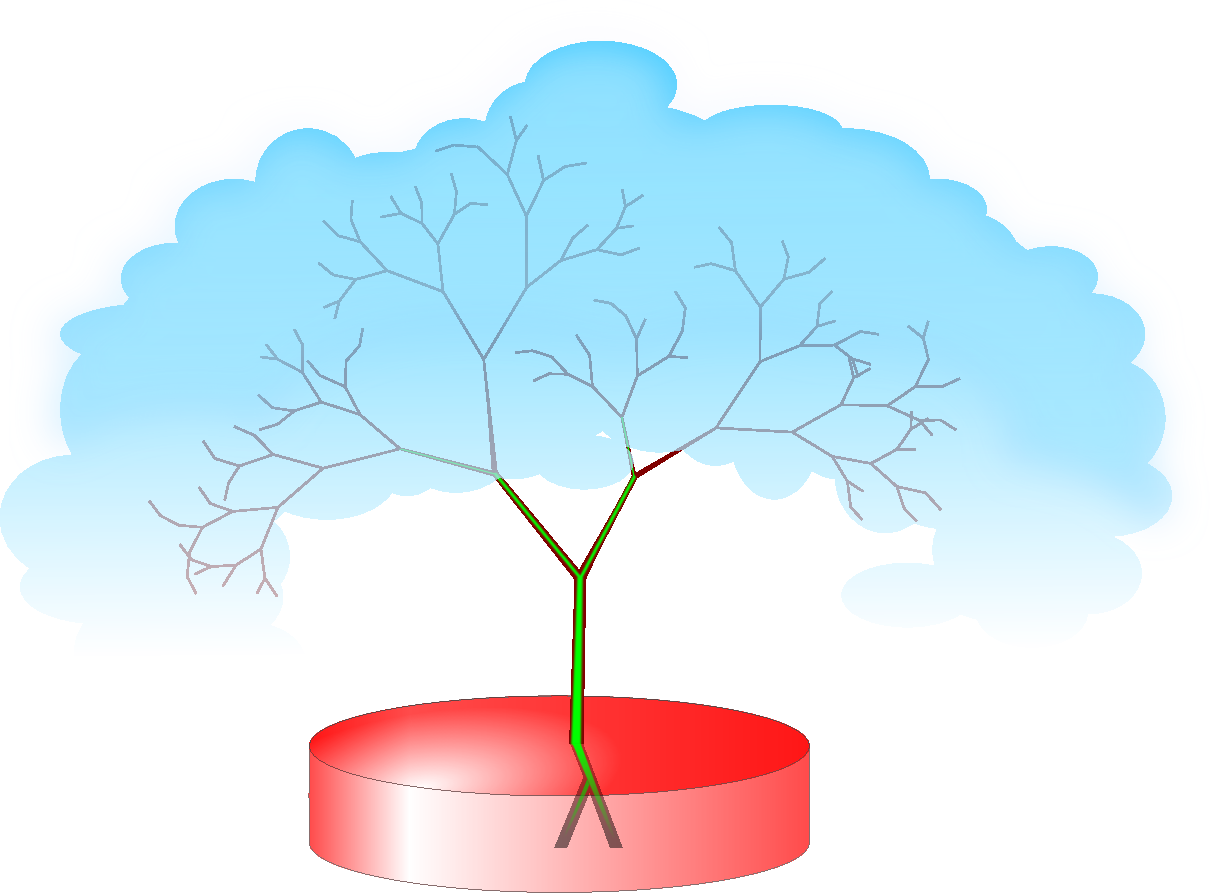
\includegraphics[width=7cm]{complete.pdf}
%\includesvg{arbornew.svg}
\end{center}
}%\\[0.4cm] % Title of your document
\HsRule \\[1.5cm]

\begin{minipage}{0.4\textwidth}
\begin{flushleft}
Giuseppe \textsc{Viola} % Your name
\end{flushleft}
\end{minipage}
~
\begin{minipage}{0.4\textwidth}
\begin{flushright}
%\emph{Supervisor:} \\
%Dr. James \textsc{Smith} % Supervisor's Name
A work carried out during the eight-month internship at the \linebreak Applied Research Team
\end{flushright}
\end{minipage}\\[3cm]

{\large June 2016}\\[3cm] % Date, change the \today to a set date if you want to be precise

%\includegraphics{Logo}\\[1cm] % Include a department/university logo - this will require the graphicx package

\vfill % Fill the rest of the page with whitespace

\end{titlepage}

%----------------------------------------------------------------------------------------
%	TABLE OF CONTENTS
%----------------------------------------------------------------------------------------

\tableofcontents % Include a table of contents

\newpage % Begins the essay on a new page instead of on the same page as the table of contents 

%----------------------------------------------------------------------------------------
%	INTRODUCTION
%----------------------------------------------------------------------------------------
\section{Prologue}
\begin{wrapfigure}{R}{7cm}\includegraphics[width=\linewidth]{prologue.png}\end{wrapfigure}
--- Hello boy, what is \A{}?\\
--- Hello sir, \A{} is a \dsel{} for the automatic generation of \ddwa{}s. It is easily extensible and...\\
--- Hold on! You're going too fast. A domain-specific what?\\
--- A \dsl{} is a computer language that is specialized to a particular application domain. It's not like C, or Lisp, which you can use to build pretty much what you want. It's like SQL for database queries, or HTML for web pages.\\
--- Hmm, I see. But tell me more about generation: you mean that you're actually \emph{generating} working code?\\
--- Yes, I am. You know, the concept is not new at all: that's what compilers do. If you see a C program as a data structure, then you can manipulate it as you like. For example, you can transform it to machine code. The key point here is \emph{program as data}. Imagine you are able to represent a class of problems using a data structure. Then I can provide you with a language and a translator. You use the language to specify in a simple way the problem that you want to solve. Then you launch the translator, and you have your code!\\
--- Sounds too good to be true. Where's the catch?\\
--- You're right, there's a catch, indeed. Or, better, a trade-off, like everything else in engineering. If you want to describe a whole application in a simple way, then you're bound to lose some fine control over it. I'll give an example from the compiler world, again: if you are willing to lose the power of specifying exactly what CPU registers should hold which variables, then you can write your program in a more convenient, high-level language like Java (instead of the nightmarish assembly) and you let the compiler fiddle around with the register allocation...\\
--- So, in a few words, you're proposing to use a small language, not suitable for a general piece of software, to build a whole application. That way you keep the development simple, and your translator takes care of the real code synthesis, like a compiler.\\
--- Exactly! But that's not the whole story, sir. Alongside the code generation, you can produce a lot of other artifacts that generally require a tremendous effort from the developers. Think about it: what prevents you from using this trick to produce software documentation too? If you properly annotate your specification with well formed comments, it is possible to produce the kind of boilerplate documentation that nobody wants to write --- think to the tons of pages necessary to go over the details of a REST API. You can produce a video user manual of your application, with synthesized speech that illustrates how it works. You can also generate test code: you know how long it takes to write test cases for a client-server application, don't you?\\
--- Hmm, I still believe this is like open eyed dreaming, boy.\\
--- Well, so do I... That's why I've been playing around with those concepts and built \A{}. It is a language for the specification of simple \ddwa{}s. You know, things like database access masks, data entry and visualization, chart rendering, and so on. If it works, it will give me some adrenaline to keep on believing that there can be a software developing environment where you modify things only in one place, and the rest will update instantly and consistently.\\
--- Ok boy, I admit you intrigued me. I'll sit here, and listen to what you have to say...
\newpage
\section{Introduction}
The history of computer science is permeated with the concept of abstraction. Since the very beginning, computer scientists and practitioners endeavored to build successive layers of progressively abstract concepts, with the twofold purpose of reusing previous work and facilitating design. Examples range from the stack of computer network communication protocols, to the implementation of operating systems, and to the layers of database design. But perhaps the area of computer science that benefited most from this paradigm is the design of programming languages. The past 60 years saw the astonishingly rapid evolution from the first machine code programs to the plethora of high level languages and frameworks that populate today's computer world. The propeller of such a process has always been the desire for an easier --- and less error prone --- development of software systems; this evolution is still at work today, with the global cost of bug-fixing totalling more than \textdollar{}300 billion per year\footnote{See Cambridge University's study results at \scriptsize\url{http://www.prweb.com/releases/2013/1/prweb10298185.htm}}. 
The propeller, in turn, has been fueled on the abstraction paradigm: citing Wikipedia's page on abstraction in software engineering\footnote{See \scriptsize\url{https://en.wikipedia.org/wiki/Abstraction_(software_engineering)}}:
\begin{shadequote*}
%\begin{flushright}
   \emph{In discussing formal semantics of programming languages, \\
   abstraction refers to the act of considering a less detailed, \\
   but safe, definition of the observed program behaviors.}
%\end{flushright}
\end{shadequote*}
%\rightline{\emph{In discussing formal semantics of programming languages}}
%\rightline{\emph{abstraction refers to the act of considering a less detailed,}}
%\rightline{\emph{but safe, definition of the observed program behaviors.}}\\
Many roads exist to reify such a spirit, that is, relieving the designer from the burden of specifying too many details. Over the past years, for instance, the web world showed great interest towards the definition of frameworks that spared designers from programming the tiniest bits of their web applications. 

That very same spirit drove the development of the \A{} language, although on a slightly different road. \A{} belongs to the vast family of \dsl{}s\cite{dslannot}:

%\begin{tcolorbox}[colback=cyan!5!white,colframe=blue!75!black,title=\Dsl{}]
%\begin{shadequote*}
\q{A \dsl{} is a programming language or executable specification language that offers, through appropriate notations and abstractions, expressive power focused on, and usually restricted to, a particular problem domain}.
%\end{tcolorbox}
%\end{shadequote*}

\A{}'s domain is the realm of data-driven web applications, but \dsl{}s have been defined for almost any sector. Interesting surveys on the subject may be found in \cite{dslannot}, \cite{dsltheor}, which offer a detailed analysis of the advantages and drawbacks of their use in a production context.
It is not the purpose of this document to delve into those topics. Rather, here the \DSL{} approach is embraced, with the following goal:
\begin{tcolorbox}[enhanced,title=Goal,fonttitle=\bfseries,
colframe=blue!50!black,colback=blue!10!white,colbacktitle=blue!5!yellow!10!white,lifted shadow={1mm}{-2mm}{3mm}{0.1mm}{black!50!white},fonttitle=\bfseries,coltitle=black,attach boxed title to top center=
{yshift=-0.25mm-\tcboxedtitleheight/2,yshifttext=2mm-\tcboxedtitleheight/2}]
Build a prototype \dsl{} for the design of \ddwa{}s, to prove the feasibility of \DSL{}-driven engineering of software systems characterized by recurring patterns, architectures, and data abstractions.
\end{tcolorbox}
~\\
As an example, consider a specialized team of a large IT institution, devoted to the realization and maintenance of web front ends for customers spread all over the globe. The vast majority of such front ends, on one hand, may share the same data abstractions, the same programming patterns, the same logical architecture. On the other hand, they may be coded in different languages, due to the cited abundance of web frameworks, or they may use different data access primitives, to be interoperable with legacy systems. In this context, a \DSL{} may help in two ways: first, by factoring out the commonalities, and providing a \q{less detailed, but safe} specification of recurring operations, often in a fully \emph{declarative} fashion; second, by abstracting away all the low-level implementation differences, and exposing a \emph{universal} and \emph{extensible} way of handling them. Here, emphasis has been put on the words declarative, universal and extensible: each of them plays an important role in the design of \A{}, and will be detailed in their own box.

This document provides an outline of \A{}'s design and characteristics. It is organized in two main parts: the first, and more substantial one, details the design choices that drove the development of the \A{} language. Then comes a less detailed part about the implementation aspects of the translator. The decision of not providing the minutiae of the translator coding comes from the consideration that it is just one of several possible implementations, targeted towards a specific output language. Changing the target language would entail a refactoring of the translator, whereas the specification language itself would remain unaltered.

\section{\A{} design}\label{design}
This section will focus on the design choices and implementation details of the \A{} language. \A{} is a \dsel{}, having \Hs{} as the host language. It defines a set of primitives for building \ddwa{}s.
The design choices are presented \q{from the ground up}, by exploiting the analogy between the \A{} logo and a tree. As a matter of fact, each part of the tree symbolizes one or more design choices, as it will become apparent later on.

\subsection{The ground}\label{ground}
The first design choice made in \A{} is the precise definition of its \q{problem domain}:
\marginpar{\vspace{3cm}\begin{flushleft}\scriptsize The ground is the usual symbol representing a relational database\end{flushleft}}
\begin{dce}{\Ddwa{}s}{dd}{noroot.pdf}
A \ddwa{} is a client-server application focused on the treatment and visualization of data in relational form, in which:
\begin{itemize}
\item the \fe{} is an HTML/Javascript page, accessible from a standard web browser 
\item the \be{} is a remote web service. 
\end{itemize}
The application user may create, read, update and delete data resources by using all common HTML controls, such as input fields, drop downs, labels, images, vector graphics, buttons, and so on.
\end{dce}
~\\
Thus, an \A{} program is, to all effects, a single-page web applications that interacts with a remote server. The language offers the primitives to build such an application, and the translator produces the actual HTML/Javascript code to be rendered by the browser.

Here, a question may come naturally: why the focus on relational data, and what is excluded from \A{}'s problem domain?

The relational data model has been the most used data model in the past years, and it still is today, even though nonrelational models are growing their market share. It is the model that large IT enterprises have hardcoded in their mainframes, and that many web applications have to deal with. Therefore, the design choice made here means that the designers will have to think about their data in terms of tables and queries. In \A{}, it is not possible to design data in graph form, or in object-oriented pointer-based fashion. This excludes from the applications that can be written in \A{} all those whose data layer is too convoluted to be easily expressed in relational form, or whose interaction with the user requires more sophisticated (non-HTML) controls. 


\subsection{The roots}\label{roots}


Several times, in the previous sections, \A{} has been given the attribute of being \emph{embedded}.
This is the second design choice:
\\
\marginpar{\vspace{0.5cm}\begin{flushleft}\scriptsize The root is a stylized lambda, the symbol for \Hs{} and all functional languages built on the $\lambda$-calculus.\end{flushleft}}
\begin{dce}{Domain-specific \emph{embedded} language}{lambda}{nobranches.pdf}
\vspace{1cm}
\A{} is a deeply embedded \dsl{} having \Hs{} as host language.
\vspace{1cm}
\end{dce}
~\\
Citing \cite{elliott}, \q{the essential idea [of an embedding] is to augment a host programming language with a domain-specific library. Modern functional host languages are flexible enough that the resulting combination has more the feel of a new language than a library. Most of the work required to design, implement and document a language is inherited from the host language}.

In other words, \A{} code is just plain \Hs{} code, built using predesigned functions and operators.
Such code produces an intermediate \Hs{} data structure, resembling an \abs{} (\ABS{}) (it actually contains additional information, as it will be clear later). Such a data structure is then input to the translator, which outputs the required HTML/Javascript code.

The choice of embedding \A{} into \Hs{} comes from the advantages in terms of easiness of parsing. There is no need to specify a dedicated grammar, with all issues of operator precedence and associativity. \Hs{}'s grammar and its compiler takes care of everything. Moreover, static type checking ensures that only well formed expressions and elements can be accepted and translated into target code.

The attribute \emph{deep} is of purely technical merit: deep and shallow embeddings differ in the way they use the host language \abs{}. In a shallow embedding, the language constructs directly produce expressions in the host language \ABS{}. In a deep embedding, as already stated, an intermediate custom \ABS{} is used. Both choices have their own pros and cons, of course; here the latter choice has been made, because it offers more control on the intermediate data structure, in terms of further semantic checks and optimization that can be performed before the actual translation into the target language takes place.

It is time now to introduce the first of the three key features of \A{} code cited in the Introduction: declarativity.\\

\begin{kfe}{Declarativity}{declarativity}
\A{} code is declarative in the sense that it specify \emph{what} elements the application is composed of, and \emph{what} computations, actions, and transitions those element are subject to, without specifying \emph{how} they are carried out. In other words, the language abstracts over all the underlying details, and provides the users with a simpler and more readable way to design their applications, closer in a sense to their natural language description.
\end{kfe}
~\\
Key feature \ref{declarativity} refers to a natural language description of the application. This is generally the first stage of the design of any application: it may be a requirement document, a scratch on a piece of paper, or even just a thought. The purpose of a \DSL{} is to bring such a description and a working implementation closer together. 
The following sections will outline how this objective can be reached. Here, an example of this natural language description will be scratched, to become the running example throughout the rest of the document:\\
\begin{tcolorbox}[colback=yellow!5,fonttitle=\bfseries,colframe=yellow!50!black,title=Description of a webshop application in natural language,lifted shadow={1mm}{-2mm}{3mm}{0.1mm}{black!50!white}]
\myverb{\scriptsize The interface screen area should show either the login form or the main application page.\newline
The main application page, then, should be subdivided in two sections: a navigation bar on the left, and a large central area.\newline
The navigation bar could be either in standard mode, showing only some action buttons, or in expert mode, showing all possible action buttons.\newline
The large central area, in turn, could show many different views, depending on the application state: the welcome screen, to be shown upon entering from a successful login, with its product search form; or a list of all product details resulting from the search; or a dashboard containing aggregate cart data for subsequent processing and payment.\newline
More in detail, each element of the product list should contain, from left to right, labels showing name, brand and price, a picture, and a \q{buy it} button.}
\end{tcolorbox}

\subsection{The branches}\label{branches}
This section introduces the language tools used by the designer to build the user view of the application. In a typical web application, a user view is composed by sequences of simple elements like buttons, labels, and input fields, arranged in a certain graphical layout (horizontal or vertical). Such elements may then be grouped in more complex elements such as forms or lists. Furthermore, the same screen area may display different sets of elements, depending on the situation. These considerations led to the need of expressing in a simple way elements of increasing complexity, which could be sequenced, grouped and alternated. The theoretical word for expressing this concept is \emph{inductive definition}:\\
\begin{dce}{Inductive definition of elements}{element}{nolymph.pdf}
The user view is specified in terms of elements. An element can be either: 
\begin{description}
\item[Simple] a simple HTML control (like a button, an input field or a label)
\item[Sequence] a sequence of elements, laid out horizontally or vertically
\item[Container] a container of elements (like a list)
\item[Choice] a choice of exactly one element from a map of elements. The map, indexed by a name, groups together all elements that share the same screen area. The elements contained in the map may optionally be parametric, that is, their actual content may depend on the value of some input parameters.
\end{description}
\end{dce}
~\\
\marginpar{\vspace{-7cm}\begin{flushleft}\scriptsize The inductive definition of element is depicted as the tree branches\end{flushleft}}
The actual design of a user view can be carried out in both top-down and bottom-up fashions, through the use of custom operators that permit, for instance, to lay elements horizontally, or to build the choice map. More details on such operators will be given soon.

The inductive definition of an element implicitly carries an important consequence: a user view can be represented as a tree of elements, having as root the user view as a whole, and a multitude of simple HTML controls as leaves. All non-leave nodes represent either a sequence, a container or a choice of child nodes. They are called sequence, container or choice nodes, respectively. In the latter case, each child node is uniquely identifiable with its corresponding name in the choice map.

Design Choice \ref{element} gives great freedom in specifying the user view. In particular, the top-down specification process may closely resemble the natural language specification of Section~\ref{roots}. As an example, here follows the \A{} code for specifying a portion of the user view of the webshop application:\\

\begin{tcblisting}{enhanced,lifted shadow={1mm}{-2mm}{3mm}{0.1mm}{black!50!white},fonttitle=\bfseries,colback=yellow!5,colframe=yellow!50!black,listing only,title=Specification of a webshop application in \A{},fontlower=\sffamily\bfseries,listing engine=minted,minted language=haskell,minted options={fontsize=\fontsize{7}{8}\selectfont,linenos,numbersep=3mm}}
interface = do
    l <- login
    h <- home
    a <- alternative [ l <@> "login", h <@> "home" ]
    return a
    
login = do 
    userid  <- input (string "user id") 
    passwd  <- input (string "password")
    ok      <- button (string "login")
    return $    userid
            <-> passwd
            <-> ok
            
home = do 
    ns <- navbarstd
    ne <- navbarstd
    w <- welcome
    p <- results
    c <- cart
    a1 <- alternative [ ns <@> "navbarstd", ne <@> "navbarexp "]
    a2 <- alternative [ w <@> "welcome", p <@> "results", c <@> "cart" ]    
    return $ a1 <|> a2
    
navbarstd = do
    wb <- link "welcome" 
    cb <- link "cart" 
    lb <- link "logout"
    nb <- navbar [wb,cb,lb]
    return nb
    
welcome = do 
    lab <- label (string "Filter product")
    inp <- input (string "")
    btn <- button (string "go")
    return $    lab <|> inp
            <-> btn
            
results = do
    par <- parameter "search"
    let showProduct prod = do
            ln <- label (prod ! "name")
            lb <- label (prod ! "brand")
            lp <- label (prod ! "price")
            li <- image (prod ! "image")
            b  <- button (string "buy it")
            return $ ln <|> lb <|> lp <|> b 
	prodList <- list (searchProducts par) showProduct
    lab <- label (string "Filter results")
    return $ par <\> lab
                 <-> prodList
\end{tcblisting}
\pagebreak
The specification of an element is divided into three parts\footnote{The \myverb{do} notation is specific to \Hs{}: it introduces monadic code (see Section~\ref{monads}). Here, it can be regarded as a syntactical nuisance coming from the choice of embedding \A{} into \Hs{}. From the designer point of view, the \Hs{} keywords \myverb{do} and \myverb{return} may be regarded as code block delimiters.}:
\begin{enumerate}
\item Declaration of the \textbf{main element} name (left hand side of the assignment introduced by '\myverb{=}')
\item Declaration of all the \textbf{constituting elements} (statements enclosed by \myverb{do} and \myverb{return})
\item Declaration of the \textbf{element layout} (\myverb{return} statement)
\end{enumerate}

A constituting element declaration is formed by the element name, the arrow operator '\myverb{<-}' and the right hand side, which can be either the name of another main element, or a simple element (like \myverb{label}, \myverb{input} and \myverb{button}), or a container element (like \myverb{list}). In either case, appropriate arguments are passed to these constructs, like initialization strings for simple elements, or element layouts in case of containers. 
An element layout is defined by grouping elements together with the layout combinators:
\begin{description}
\item \myverb{<|>} (horizontal layout combinator): this combinator puts two elements side by side
\item \myverb{<->} (vertical layout combinator): this combinator stacks the two elements one above the other
\end{description}
An element layout is also the argument of the \myverb{return} keyword. Such layout is identified then by the element name given in the first line of the code block. 

The \myverb{list} element deserves particular attention: it is here that functional languages like \Hs{} show most of their power. The call to \myverb{list} takes as arguments the query \myverb{(searchProducts par)} (see Section \ref{query}), and the \emph{function} \myverb{showProduct}. Such a call means that the function must be called for each record retrieved by the query, and its result displayed in the user view. The \myverb{showProduct} function, in turn, is defined in the \myverb{let} expression as a function of the \myverb{prod} record, and gives as output a horizontal concatenation of five simple elements showing product information. It is very easy, then, to build lists out of queries, considering that such list calls may be nested to build smaller lists inside bigger ones (e.g. list of all customers, for each of which all telephone numbers are displayed).

The detailed description of the \A{} syntax will not be pursued further here. What has been shown has the purpose of demonstrating the declarativity of the \A{} code: the designer specifies only what the user view is constituted of, and its layout arrangement. The physical separation between the declaration of constituents and that of their layout is a crucial aspect of the design of \A{}. Later it will be pushed even further, upon the introduction of the concept of application state. In the next section, indeed, the application state will be \q{injected} into the element tree structure, thus bringing life to the skeleton built here, through the concepts of \emph{poses} and \emph{transitions}.\\


\subsection{The lymph}\label{lymph}
So far, the tree of elements is just about the skeleton of an application. The next step is to define its dynamics, namely, what elements are currently shown to the user, when and how it responds to user inputs and the deriving actions, and so on. In a word, there is the need of specifying its behavior. Towards that end, a true cornerstone is represented by the concept of application state:\\

\begin{dce}{\Fe{} as a Finite State Machine}{fsm}{nocrown.pdf}
The whole \fe{} can be thought of as a Finite State Machine (FSM), with each state corresponding to the view currently displayed in the \wb{}. The application designer specifies what each state is made of, and what transitions towards other states are allowed, optionally specifying a side-effecting action to be performed --- typically, a user alert or a \be{} request. In other words, the application state is a subtree of the element \abs{}.
\end{dce}
~\\
Having in hand the inductive definition of element given in Section~\ref{branches}, it is easy to identify the application state with a subtree. Indeed, at any given instant, only a portion of the whole tree is visible to the user. Its visible elements are determined by the choices made at the choice nodes (one among the alternatives) and their content may be also influenced by the parameter values. 
At this point, a new language construct is required to identify such a subtree, which is able to keep track of all decisions made at the choice nodes, together with their parameter values. Such a construct is called \emph{pose}, and can be thought of as a generalization of the concept of URL. In the same spirit as the element, also the pose is defined inductively:\\
\begin{dce}{Pose}{pose}{nocrown.pdf}
A pose is either:
\begin{description}
\item[Segment] a segment consists of a name and, when applicable, a list of parameter values: the name is used to index the choice map of a choice node
\item[Concatenation] the concatenation of a segment and another pose, to represent choices made at nested choice nodes
\item[Tuple] a tuple of poses, to represent the multiplicity of choices that have to be made when a sequence node contains more than one choice node
\end{description}
\end{dce}
\marginpar{\vspace{-5cm}\begin{flushleft}\scriptsize The pose is symbolized by the green lymph that highlights some of the branches\end{flushleft}}
~\\
Analogously to elements, pose combinators have been defined to ease their specification:
\begin{itemize}
\item \myverb{seg} (segment combinator): produces a segment pose from a name and a list of parameters
\item \myverb{</>} (concatenation combinator) : produces a concatenation pose from a segment and another pose
\item \myverb{<\&>} (tuple combinator): produces a tuple from two poses
\end{itemize}

An example will clarify the definition: the pose 
\[
\myverb{seg "home" [] </> (seg "navbarstd" [] <\&> seg "welcome" [])}
\]
corresponds to showing the user the home page (instead of the login one); in turn, the home page contains the standard navigation bar (instead of the expert one) and the welcome page (and not the products or cart ones).

Going back to Design Choice \ref{fsm}, it is clear now that each state of the FSM is uniquely identified by a pose.
It remains to define what the edges are made of: it is the purpose of the next design choice.
\\

\begin{dce}{Transition}{sep}{nocrown.pdf}
A transition between two application states is defined in terms of three items (referred to as EAT items):
\begin{description}
\item[Event] an event occurs when the user interacts with one of the visible elements, like clicking on a button, or hovering on a list element
\item[Action] an action may be performed during the transition, like updating an internal table or submitting a form to the \be{}
\item[Target] the target application state that the transition reaches after performing the action: the target state is specified by a pose whose parameter values may be determined by the values of the visible elements.
\end{description}
\end{dce}
~\\
Transitions can be specified for any element by providing their EAT items in their declaration blocks. As an example, the code written in Section~\ref{branches} will be rewritten now with the transitions added\footnote{For space reasons, some details have been left out, such as the action performed upon login (verification of user credentials).}:\\
\begin{tcblisting}{enhanced,lifted shadow={1mm}{-2mm}{3mm}{0.1mm}{black!50!white},fonttitle=\bfseries,colback=yellow!5,colframe=yellow!50!black,listing only,title=Specification of state transitions,fontlower=\sffamily\bfseries,listing engine=minted,minted language=haskell,minted options={fontsize=\fontsize{7}{8}\selectfont,linenos,numbersep=3mm}}
[...]
login = do 
    userid  <- input (string "user id") 
    passwd  <- input (string "password")
    ok      <- button (string "login")
    transition ok click none 
       (seg "home" [] </> (seg "navbarstd" [] <&> seg "welcome" []))
    return $    userid
            <-> passwd
            <-> ok
[...]
welcome = do 
    lab <- label (string "Filter product")
    inp <- input (string "")
    btn <- button (string "go")
    transition btn click none 
        (seg "home" [] </> 
            (seg "navbarstd" [] <&> seg "results" [("search",value inp)]))
    return $    lab <|> inp
            <-> btn
[...]
results = do
    par <- parameter "search"
    let showProduct prod = do
            ln <- label (prod ! "name")
            lb <- label (prod ! "brand")
            lp <- label (prod ! "price")
            li <- image (prod ! "image")
            b  <- button (string "buy it")
            transition b click 
                (command insertProduct cart)
                (seg "home" [] </> (seg "navbarstd" [] <&> seg "cart" []))
            return $ ln <|> lb <|> lp <|> b 
	prodList <- list (searchProducts par) showProduct
    lab <- label (string "Filter results")
    return $ par <\> lab
                 <-> prodList
\end{tcblisting}
~\\
It is easy to identify the EAT items in the previous code fragment. Particular attention must be given to the pose relevant to the transition present in the \myverb{welcome} element, which gives sense to the choice of having parametererized elements in choice nodes. Here, the necessity of carrying around the information of the search string input by the user in the welcome page has been coded into a parameter passed to the \myverb{results} element. It is the \myverb{results} element itself that  takes care of properly exploiting this piece of information, by using it in the \myverb{searchProducts} query.


\subsection{The crown}
Last, after building on roots and branches, comes the design choice that closes the gap between the \fe{} and the \be{}. It disciplines the design of their interaction, in terms of feasible operations that may be performed. \\
\begin{dce}{RESTful interaction}{rest}{complete.pdf}
The interaction between the \be{} and the \fe{} is inscribed into the REST framework. It is assumed that the \be{} exposes a RESTful API, in terms of Create, Read, Update, Delete operations on its resources and collections thereof.  The \fe{} may issue one of those operations in the following ways:
\begin{description}
\item[Create] a resource in a remote collection, for instance by submitting the contents of a form, or uploading an internal table after manipulating it through several application states
\item[Read] the contents of a resource or a collection, typically upon entering an application state containing elements with content dynamically retrieved from the \be{}
\item[Update] a resource, for example by uploading an internal table previously filled with content coming from the \be{} and modified through several application states
\item[Delete] a resource when it is no longer needed
\end{description}
\end{dce}

\marginpar{\vspace{-8.3cm}\begin{flushleft}\scriptsize The tree crown symbolizes the REST interaction between the application and the \emph{cloud}\end{flushleft}}
~\\
This design choice constrains the actions that may be performed in response to events. Basically, no remote procedure calls are allowed, and the design of the application states must reflect the way the \be{} APIs are designed.

\section{Implementation}\label{implementation}
This section deals with the details of the \Hs{} implementation of the \A{} translator. Some of the techniques used will be presented in their own short section, with the purpose of giving a glimpse of the machinery underlying the implementation of a \DSL{} translator.

\subsection{Monads}\label{monads}
Monads are one of the most useful programming techniques in the \Hs{} world. There are plenty of ways of giving a definition of what a monad is, but for the purpose of this document, a monad will be thought of as a way of wrapping a context around a computation. Haskell itself utilizes monads at its very heart to perform IO in a safe and referencially transparent way. Such contexts may be of different nature: some, like IO, Error, State, are predefined. Others may be created by the programmer, provided that some Monad Laws are satisfied. Either way, all monads may be composed (i.e. stacked) to build context of increasing complexity, whenever they are needed.

The \A{} translator uses monads in three different places:
\begin{enumerate}
\item The language \fe{} is wrapped in a State monad, which is used as a supply of fresh names for uniquely identifying the elements of a user view, and to store the Transition table
\item The Query language (see Section~\ref{query}) uses a custom Query monad, very similar to a State one, to progressively store the query that is being built by the user using a sequence of commands
\item The generator uses a Reader monad, to provide local context to each code generating routine (e.g. the path in the element tree identifying the view that the current element belongs to, the container that might include it, etc.)
\end{enumerate}

\subsection{Query language}\label{query}
The binding between visualization and data is represented by the query language. As already pointed out in Section~\ref{ground}, data is abstracted using the usual relational paradigm: it is structured into records with primary and foreign keys, and records are grouped into tables, which can be local to the client, or stored on the server as REST collections. As a consequence, the need emerges for a query language, able to perform all standard relational operations, such as selection, projection and product. Instead of resorting to the SQL language, known to be not type safe, a mini \dsl{} has been developed, inspired by \cite{leijen}. A query is represented by a list of statements in the Query monad, that incrementally build the \abs{} of the output relation. Such \abs{} is then used to generate the Javascript code necessary to perform the required operations. In other words, a small relational engine is embedded in the application code, that is responsible for all the binding between view and data.
As an example, consider what the query for showing the user a list of products might be in the webshop application:\\
\begin{tcblisting}{enhanced,lifted shadow={1mm}{-2mm}{3mm}{0.1mm}{black!50!white},fonttitle=\bfseries,colback=yellow!5,colframe=yellow!50!black,listing only,title=An example of \A{}'s query language,fontlower=\sffamily\bfseries,listing engine=minted,minted language=haskell,minted options={fontsize=\fontsize{7}{8}\selectfont,linenos,numbersep=3mm}}
searchProducts param = do 
    prod <- table products
    restrict (prod ! "name" *==* param)
    project [ "name"  *@* "prodName"
            , "brand" *@* "prodBrand"
            , "price" *@* "prodPrice"
            ]
\end{tcblisting}
~\\
The query is built using three commands:
\begin{enumerate}
\item The \myverb{products} table is referred to, and \q{loaded} into the Query monad; furthermore, its scheme is saved in the \myverb{prod} variable
\item The records showing a \myverb{name} attribute equal to the input paramenter \myverb{param} are selected from the table; the resulting table is saved in the Query monad 
\item the \myverb{name}, \myverb{brand} and \myverb{price} attributes are projected and renamed. Again, the result is saved in the monad and returned to the calling function.
\end{enumerate}
The query language implemented in \cite{leijen} is equivalent in power to SQL. in \A{} only a subset with limited functionalities has been implemented for the time being, but its extension to support all SQL constructs should be straightforward.
\subsection{Pose parser}
The adoption of the concept of pose to represent the application state brought the problem of its encoding inside the target Javascript \fe{} code. Due to lack of native \adt{}s in Javascript, the choice has fallen back to encoding a pose as a string. This, in turn, entailed the necessity of implementing a grammar and its parser.
Following \cite{aho}, an L-attributed, right recursive grammar has been designed, and the relevant parser has been implemented through recursive descent with one symbol of lookahead. The syntax-directed translation gives as output the list of all element paths that make up the pose.
\subsection{Target language}
As mentioned in Section~\ref{ground}, the target language chosen for the current implementation of the \A{} translator is HTML/Javacript. In particular, the Javascript code makes use of the Angular JS framework. Such a choice has been made based on the popularity of the framework itself and on the easiness of code generation. More in detail, the \A{} translator creates an isolated-scope directive for each choice element present at choice nodes and for all list containers. Each directive has associated an HTML template and a controller. Such a choice shown to be very effective from the point of view of translator implementation. Indeed, every element is responsible of generating its own code, in terms of directives, templates and controllers, based on the current context provided by the Reader monad. This is one key aspect, further explored in Key Feature \ref{extensibility}.\\

\begin{kfe}{Extensibility}{extensibility}
The extensibility of a \dsl{} is of primary importance in a continuously changing environment: as a general statement, the addition of new commands and expressions puts pressure on the translator developers, who are asked to extend the \DSL{} to support the new needs. A truly extensible \DSL{} allows one to add new features without \emph{any} modification to the existing code base --- the notorious expression problem\cite{reyn}. \Hs{}'s typeclasses elegantly addresses such an issue, allowing the addition of new elements (widgets, containers, etc.) to \A{}'s expressive power without touching any of the existing translator code.
\end{kfe}
This attribution of responsibility to each element in defining their own generated output brings another positive consequence. If generated code is needed in another target language, it suffices to refactor only the translator backend code to reflect the new target peculiar features. This is Key Feature \ref{universality}.\\
\begin{kfe}{Universality}{universality}
Universality of the \A{} language refers to the possibility of using the unaltered specification language as the input to a totally different translator, to produce, say, Java/Swing code instead. Here resides the power of the \DSL{} approach: a true decoupling between the language used to specify a piece of software, and the underlying implementation language. As far as \A{} is concerned, web frameworks may come and go, as well as standalone GUI libraries, but the translator can be readdressed to different target languages, to reflect the specific needs. That way, the application portfolio can migrate to the new technology through a new translation, together with its documentation and test code.
\end{kfe}

\section{Generation artifacts}
The expressive power of a high-level \DSL{} like \A{} makes it possible to centralize the development of a web application in only one place, namely the \A{} source code. With little effort, such a place may become the only one that needs to be modified, extended, or maintained. It could truly represent an \emph{executable specification}, from which not only the target code is derived, but a large bouquet of artifacts may be produced. An exercise has been made, for instance, to derive a \q{video user manual} of the generated application, by means of the custom scripting language AutoHotkey\footnote{See \scriptsize\url{https://autohotkey.com/}.}. The starting point is, as usual,  the \abs{} representing the whole user view, together with the transition map. Then, the Finite State Machine of section \ref{lymph} is built, and a depth-first visit is performed to touch all of its nodes and walk all of its edges. During the visit, AutoHotkey code is generated to simulate mouse clicks and keyboard strokes aimed at showing the interaction with each element of the user view. 

To help the process and give clearer description of all elements, a new operator \myverb{<?>} has been defined to let the user annotate the \A{} source code with suitable comments. For instance, annotating the \myverb{login} element would result in the following code:\\

\begin{tcblisting}{enhanced,lifted shadow={1mm}{-2mm}{3mm}{0.1mm}{black!50!white},fonttitle=\bfseries,colback=yellow!5,colframe=yellow!50!black,listing only,title=Code annotation for documentation generation,fontlower=\sffamily\bfseries,listing engine=minted,minted language=haskell,minted options={fontsize=\fontsize{7}{8}\selectfont,linenos,numbersep=3mm}}
login = do 
    userid  <- input (string "user id")  <?> "Here the user enters their id"
    passwd  <- input (string "password") <?> "This is the password field"
    ok      <- button (string "login")   <?> "Clicking this button triggers
                                              the credentials verification"
   transition ok click none 
       (seg "home" [] </> (seg "navbarstd" [] <&> seg "welcome" []))
    return $    userid
            <-> passwd
            <-> ok

\end{tcblisting}
~\\
Such annotations may also be used to generate written documentation, for instance in HTML or pdf form. 
Another artifact that may be automatically generated with similar considerations is test code. Both unit and end-to-end tests could be produced from the \A{} source code. For unit tests, each case would contain acceptable and nonacceptable (random) user inputs whose generation is based on the characteristics of the specific element to be tested. End-to-end tests would produce code that makes the \fe{} and the \be{} interact at various time rates, or in burst form. 

In each of the aforementioned examples, the only place holding the application design information is the \A{} code. No replication or fragmentation, then, may cause missing or inconsistent content in generated artifacts.
\section{Conclusions}
\A{} is an example of a language for layered software engineering. This document described its design choices, and pointed out its key features. The Goal presented at the beginning was ambitious: time will tell if \A{} is suited for it, and when and how it should be modified or extended. A possible penetration strategy for its adoption could be to use it as a language for early stages of web application development, that is, for the rapid prototyping of first releases. Its use in this kind of context would help pointing out design flaws and possible improvements, in terms of language capabilities and implementation performances. As a general statement, \A{} may also represent an example of applicability of the \DSL{} paradigm to other development areas.
\newpage
\section{Epilogue}
\begin{wrapfigure}{R}{7cm}\includegraphics[width=\linewidth]{epilogue.png}\end{wrapfigure}
--- Ok, boy. Now I see your point. I have a question, though: how long does it take to develop and maintain the translator? I believe that the effort required is most likely larger that of the single application, isn't it? \\
--- You are right, sir. If you have to develop a single application, there's no point in devising such a contraption. But, please, think in broader terms: if you are a large firm, or a big banking institution, then it is likely that a big part of your software products will share the same architectures, design philosophies, data abstractions, and so on. It would be useful for them to invest some money in assessing whether a structured abstraction like this one could improve the whole software development process and products of that institution. That way, the cost of designing, building and maintaining the translator would spread across all the different projects, and become sustainable. \\
--- That could be one way, yes...\\
--- Sir? I have a question, too.\\
--- Go on.\\
--- Out there are many attempts at devising the perfect software development process: waterfalls, spirals, scrums are just few of the words we hear every day on the topic. Do you think there will ever be any room for \dsl{}s? I mean, large IT firms could really go bi-modal, and build a team of DSL developers. The team would  constantly be in touch with business people and customers, to seek for new or renewed requirements. Then, they would factor out the common needs, and use this knowledge to craft a \dsl{}, to be used by the application developers to produce the required pieces of software more rapidly and sustainably... \\
--- Listen, boy. Once Euclid said: \q{there is no royal road to geometry}. The same is true for software engineering: you think your approach is the way to go, others would say otherwise. You wanna know what I think? \\
--- Yes, please.\\
--- I think it's worth a try...
\newpage

\begin{thebibliography}{99}
\bibitem{dslannot} 
Arie van Deursen, Paul Klint, and Joost Visser. 2000. Domain-specific languages: an annotated bibliography. SIGPLAN Not. 35, 6 (June 2000), 26-36. 
\bibitem{dsltheor}
Domain-Specific Languages - A Theoretical Survey In Proceedings of the 3rd Compilers, Programming Languages, Related Technologies and Applications (CoRTA'2009) (2009), pp. 35-46 by Nuno Oliveira, Maria Joao Varanda Pereira, Pedro R. Henriques, Daniela da Cruz
\bibitem{elliott}
Conal Elliott, Sigbjorn Finne, and Oege De Moor. 2003. Compiling embedded languages. J. Funct. Program. 13, 3 (May 2003), 455-481.
\bibitem{leijen}
13.	Daan Leijen and Erik Meijer. Domain specific embedded compilers. In 2nd Conference on Domain-Specific Languages (DSL), Austin TX, USA, October 1999.
\bibitem{aho}
Alfred V. Aho, Ravi Sethi, and Jeffrey D. Ullman. 1986. Compilers: Principles, Techniques, and Tools. Addison-Wesley Longman Publishing Co., Inc., Boston, MA, USA.
\bibitem{reyn}
John C. Reynolds. 1994. User-defined types and procedural data structures as complementary approaches to data abstraction. In Theoretical aspects of object-oriented programming, Carl A. Gunter and John C. Mitchell (Eds.). MIT Press, Cambridge, MA, USA 13-23. 

\end{thebibliography}


%----------------------------------------------------------------------------------------

\end{document}